\chapter{Lexical and Syntactic Analysis}\label{ch:Lexical and Syntactic Analysis}

This chapter is dedicated to the development of a parser for languages generated by LR(1) grammars. The focus of this chapter encompasses the following areas: lexical analysis of the source code, testing the input grammar to check whether it's LR(1), pre-processing the source code to further facilitate parsing, and generating the derivation tree, commonly referred to as the parse tree, during parsing process.\\

The first stage of this chapter is lexical analysis, conducted by a component known as the scanner. This process involves transforming the source code, initially, a sequence of characters typically read from a file, into meaningful elements. The scanner's role is to transform these characters into lexical units, also called tokens. We will construct the lexical analyzer based on the input context-free grammar (CFG). Within the CFG framework, lexical analysis of the source code involves categorizing characters into terminal and non-terminal symbols, a process also called tokenization.\\

After reading and tokenizing of the input context-free grammar, we will check whether it's LR(1). A later step is the lexical analysis and pre-processing of the source code. During this stage, we tokenize the source code and the pre-processor cleans up the sequence of symbols derived from this tokenization process, eliminating excess elements like empty spaces, tabs, endlines, etc.\\

The final stage is syntactic analysis, executed by a parser. The parser's responsibility is to examine the sequence of symbols from the pre-processing stage and discover its hierarchical structure. The outcome of the parsing process is a derivation tree, commonly referred to as the parse tree. This tree represents the complete hierarchical structure of the source code as defined by the programming language, generated by the input context-free grammar.\\

To successfully parse the source code and to build the corresponding derivation tree, in \hyperref[sec:Structure Implementation for Context-Free Grammars]{Sect.2.1}, we implement a data structure for storing context-free grammars. Following this, in \hyperref[sec:Lexical Analysis and Tokenization]{Sect.2.2}, we read and efficiently store the input grammar. Having processed the input context-free grammar, it's time to evaluate its classification as LR(1). As Michael Sipser's book \cite{sipser} advises, we construct a \({DK_{1}}\) automaton to conduct the  \({DK_{1}}\) test. Thus, in \hyperref[sec:Structure Implementation of DK1 Automaton]{Sect.2.3}, we specify and implement the structure of a \({DK_{1}}\)\ automaton, in \hyperref[sec:DK1 Automaton Builder for a CFG]{Sect.2.4} we construct a \({DK_{1}}\)\ automaton builder for context-free grammars, and finally, in \hyperref[sec:DK1 Test]{Sect.2.5}, we run the \({DK_{1}}\)\ Test to determine whether the input grammar is LR(1).\\


After reading the source code and evaluating the input grammar's classification as LR(1), we can start the parsing process. Before this, in \hyperref[sec:Pre-processing for C0 Source Code]{Sect.2.7}, we pre-process the tokenized source code to eliminate excess elements. Now we are ready to construct the parser, but parsing without storing is meaningless, that is why first we Implement the Derivation Tree structure in \hyperref[sec:Derivation Tree Strucutre and Implementation]{Sect.2.8}, and in \hyperref[sec:Parsing and Derivation Tree Building]{Sect.2.9} we dive into Parsing and Derivation Tree Building.


\newpage


% Structure Implementation for Context-Free Grammars
\section{Structure Implementation for Context-Free Grammars}\label{sec:Structure Implementation for Context-Free Grammars}

Before diving into language ambiguity testing and the lexical analysis of the source code, we need to properly read and accurately store the input grammar. A precise specification and understanding of the source grammar are fundamental for our parser’s architecture.\\

% Context-Free Grammar Definition
\begin{definition}[1.0]
    A context-free grammar is a 4-tuple \((N, T, P, S)\), where
    \begin{enumerate}
        \item \(N\) is a finite set called the nonterminal symbols,
        \item \(T\) is a finite set, disjoint from N, called the terminal symbols,
        \item \(P\) is a finite set of production rules, with each rule being a nonterminal deriving a string of terminal and/or nonterminal symbols,
        \item \(S \in N\) is the start nonterminal symbol.
    \end{enumerate}
\end{definition}
\setlength{\parindent}{0pt}

Given this definition of a context-free grammar, our implementation will replicate its structure to properly follow the mathematical theory used in this thesis.\\

For proper replication, we create these three classes:
\begin{enumerate}
    \item Class \(\boldsymbol{Symbol}\): \textit{Both terminal and nonterminal symbols are atomic elements of CFGs. Thus, we might want to create a class that will encapsulate these elements properly.}
    \item Class \(\boldsymbol{Production}\): \textit{In CFGs, production rules dictate how a nonterminal symbol can be replaced by a sequence of terminal and/or nonterminal symbols. Therefore, we need a class that will encapsulate the concept of a production rule.}
    \item Class \(\boldsymbol{Grammar}\): \textit{This class represents the entire CFG. \(\boldsymbol{Grammar}\) should replicate the mathematical definition of CFGs.}
\end{enumerate}

For a convenient implementation design, we group these three classes under a package named \(\boldsymbol{grammar}\) - \href{https://github.com/fyfsb/dcfg/tree/main/src/main/java/grammar}{GitHub/grammar}.\\

Now let’s explore each of these classes in detail.

% Symbol Class
\subsection{Symbol Class}

The \(\boldsymbol{Symbol}\) class encapsulates the concept of terminal and nonterminal symbols. In CFGs, terminal and nonterminal symbols are strings. The input grammar explicitly determines which of the symbols are terminal and which are nonterminal. Thus, to properly encapsulate the concept of a symbol of a CFG, we need an attribute for the string content and another attribute for the type of the symbol (terminal / nonterminal).\\

\textbf{Attributes:}
\begin{itemize}
    \item \(\boldsymbol{content}\): \textit{A string representing the actual content of the symbol.}
    \item \(\boldsymbol{type}\): \textit{An enum indicating whether the symbol is a terminal or nonterminal.}
\end{itemize}

We also present some basic methods to further simplify and shorten the overall implementation of the parser.\\

\textbf{Methods:}
\begin{itemize}
    \item \(\boldsymbol{constructor}\): \textit{Initializes a \(\boldsymbol{Symbol}\) object with the specified content and type.}
    \item \(\boldsymbol{isTerminal}\): \textit{Returns true if the symbol is terminal, returns false otherwise.}
    \item \(\boldsymbol{length}\): \textit{Returns the length of the content string.}
    \item \(\boldsymbol{equals}\): \textit{Determines whether two \(\boldsymbol{Symbol}\) objects are equal in both content and type.}
    \item \(\boldsymbol{hashCode}\): \textit{Returns a hash code of the symbol.}
\end{itemize}

\begin{codeblock}[Symbol Class. Java implementation on \href{https://github.com/fyfsb/dcfg/blob/main/src/main/java/grammar/Symbol.java}{GitHub/Symbol}]
    class Symbol {
        enum SymbolType {
            Terminal, Nonterminal
        }
        String content;
        SymbolType type;

        Symbol(String content, SymbolType type) {}
        boolean isTerminal() {}
        int length() {}
        boolean equals(Object obj) {}
        int hashCode() {}
    }
\end{codeblock}

\vspace{10pt}

% Production Class
\subsection{Production Class}

The \(\boldsymbol{Production}\) class encapsulates the concept of a production rule of a CFG. A representation of a production rule has the form:

\begin{verbatim}
left (nonterminal) → right (sequence of terminals and/or nonterminals)
\end{verbatim}

meaning – the right-hand side sequence can be derived from the left-hand side nonterminal. Therefore, to properly encapsulate a production rule we need two attributes: a left-hand side nonterminal and a right-hand side sequence of symbols.\\


\textbf{Attributes:}
\begin{itemize}
    \item \(\boldsymbol{left}\): \textit{A nonterminal \(\boldsymbol{Symbol}\) representing the left-hand side of the production.}
    \item \(\boldsymbol{right}\): \textit{An Array List of \(\boldsymbol{Symbol}\) objects representing the sequence of terminals and/or nonterminals on the right side of the production.}
\end{itemize}

\textbf{Methods:}
\begin{itemize}
    \item \(\boldsymbol{constructor}\): \textit{Initializes a \(\boldsymbol{Production}\) object with the specified left and right attributes.}
    \item \(\boldsymbol{equals}\): \textit{Determines if two \(\boldsymbol{Production}\) objects are equal in both left and right.}
    \item \(\boldsymbol{hashCode}\): \textit{Returns a hash code of the symbol.}
\end{itemize}

\begin{codeblock}[Production Class. Java implementation on \href{https://github.com/fyfsb/dcfg/blob/main/src/main/java/grammar/Production.java}{GitHub/Production}]
    class Production {
        Symbol left;
        List<Symbol> right;

        Production(Symbol left, List<Symbol> right) {}
        boolean equals(Object obj) {}
        int hashCode() {}
    }
\end{codeblock}

\vspace{10pt}

% Grammar Class
\subsection{Grammar Class}

The \(\boldsymbol{Grammar}\) class represents an entire context-free grammar. Therefore, it should properly encompass:

\begin{enumerate}
    \item The start nonterminal.
    \item The terminal symbols.
    \item The nonterminal symbols.
    \item The production rules.
\end{enumerate}

That’s why we create these 4 attributes for the \(\boldsymbol{Grammar}\) class:\\

\textbf{Attributes:}
\begin{itemize}
    \item \(\boldsymbol{start}\): \textit{A nonterminal \(\boldsymbol{Symbol}\) object representing the start symbol of the grammar. By convention, it’s the left side of the first production rule of the CFG.}
    \item \(\boldsymbol{terminals}\): \textit{A set of \(\boldsymbol{Symbol}\) objects representing the terminal symbols of the grammar.}
    \item \(\boldsymbol{nonterminals}\): \textit{A set of \(\boldsymbol{Symbol}\) objects representing the nonterminal symbols of the grammar.}
    \item \(\boldsymbol{productions}\): \textit{A list of \(\boldsymbol{Production}\) objects representing the production rules of the grammar.}
\end{itemize}

\textbf{Methods:}
\begin{itemize}
    \item \(\boldsymbol{constructor}\): \textit{Initializes a \(\boldsymbol{Grammar}\) object based on the provided file path parameters:}
    \begin{verbatim} Grammar.txt, Terminals.txt.\end{verbatim}
    \textit{In order to simplify the implementation of the \(\boldsymbol{constructor}\), in the next section we will introduce other methods inside the \(\boldsymbol{Grammar}\) class.}
\end{itemize}

\begin{codeblock}[Grammar Class. Java implementation on \href{https://github.com/fyfsb/dcfg/blob/main/src/main/java/grammar/Grammar.java}{GitHub/Grammar}]
    class Grammar {
        Symbol start;
        Set<Symbol> terminals;
        Set<Symbol> nonterminals;
        List<Production> productions;

        Grammar(String grammarFilePath, String terminalsFilePath) {}
        ...
    }
\end{codeblock}

\newpage


% Lexical Analysis and Tokenization
\section{Lexical Analysis and Tokenization}\label{sec:Lexical Analysis and Tokenization}

The preceding section of the thesis introduced an efficient structure for storing a CFG. This section explores the methods to accurately read and tokenize the input grammar within this structure.\\

We provide the input grammar by passing two file paths as parameters to the \(\boldsymbol{Grammar.constructor}\):
\begin{itemize}
    \item  \texttt{Grammar.txt}: \textit{Contains the entire CFG (C0 in our case. Exactly the same representation as in \hyperref[fig:grammar_c0]{Figure 1.1}).}
    \item  \texttt{Terminals.txt}: \textit{Lists all terminal symbols. Notably, unlike nonterminal symbols, not all terminal symbols can be identified from \texttt{Grammar.txt} alone, Therefore, it’s essential to explicitly define all terminal symbols.}
\end{itemize}

The provided \texttt{.txt} files are essentially lines of strings lacking any inherent meaning. Tokenization transforms these lines of strings into sequences of \(\boldsymbol{Symbol}\) objects. We will demonstrate how to read from these \texttt{.txt} files, tokenize the content, and store it appropriately.

% readTerminals
\subsection{Grammar.readTerminals}

Parameters: \textit{String \(\boldsymbol{terminalsFilePath}\).}

Throws: \textit{\(\boldsymbol{FileNotFoundException}\) if the \(\boldsymbol{terminalsFilePath}\) is invalid.}

Returns: \textit{\(\boldsymbol{void}\).}\\

\textbf{Specification:} \textit{Utilizes \(\boldsymbol{terminalsFilePath}\) to read \texttt{Terminals.txt} and stores all terminal symbols in \(\boldsymbol{Grammar.terminals}\).}\\

Each line in \texttt{Terminals.txt} represents a terminal symbol of the input grammar. The method reads the file line-by-line, removes all whitespace to prevent unexpected errors, creates the corresponding \(\boldsymbol{Symbol}\) objects, and stores them in \(\boldsymbol{Grammar.terminals}\).

Additionally, the method adds \(\boldsymbol{Symbol}\) objects for these characters \textit{" ", "\texttt{\textbackslash t}", "\texttt{\textbackslash n}"}.

\vspace{30pt}

% readNonerminals
\subsection{Grammar.readNonterminals}

Parameters: \textit{String \(\boldsymbol{grammarFilePath}\).}

Throws: \textit{\(\boldsymbol{FileNotFoundException}\) if the \(\boldsymbol{grammarFilePath}\) is invalid.}

Returns: \textit{\(\boldsymbol{void}\).}\\

\textbf{Specification:} \textit{Utilizes \(\boldsymbol{grammarFilePath}\) to read \texttt{Grammar.txt} and stores all nonterminal symbols in \(\boldsymbol{Grammar.nonterminals}\).}\\

Each line in \texttt{Grammar.txt} corresponds to a production rule of the input grammar. As by convention at some point, every nonterminal symbol is referenced on the left-hand side of a production rule. Recognizing all nonterminal symbols requires extracting the left-hand side symbols from all production rules and storing them in the set \(\boldsymbol{Grammar.nonterminals}\).

To do this, the method reads the file line-by-line, removes all whitespace to prevent errors, splits each line at the \texttt{→} symbol, crates \(\boldsymbol{Symbol}\) object from the left-hand side of the \texttt{→}, and stores it in \(\boldsymbol{Grammar.nonterminals}\).

\vspace{30pt}

% readProductions
\subsection{Grammar.readProductions}

Parameters: \textit{String \(\boldsymbol{grammarFilePath}\).}

Throws: \textit{\(\boldsymbol{FileNotFoundException}\) if the \(\boldsymbol{grammarFilePath}\) is invalid.}

Returns: \textit{\(\boldsymbol{void}\).}\\

\textbf{Specification:} \textit{Utilizes \(\boldsymbol{grammarFilePath}\) to read \texttt{Grammar.txt} and save all production rules in \(\boldsymbol{Grammar.productions}\).}\\

As mentioned earlier, each line in \texttt{Grammar.txt} represents a production rule of the grammar. Sometimes, the symbol \texttt{|} is used to represent multiple productions on the same line when the left-hand side nonterminal is identical for those right-hand sides of the productions.\\

Example: \texttt{S → a | b}

For proper implementation, we should decompose such representations and store each production separately.\\

Instead of,  \texttt{S → a | b}, we should store,  \texttt{S → a; S → b}, separately.\\

To do so, we split each string line by  \texttt{→}. Then we create a variable, \(left\), which is a \(\boldsymbol{Symbol}\) object obtained from the left-hand side string. We save the right-hand side string as  \(rightString\). To decompose  \(rightString\), we split it by \texttt{|} and store the resulting parts in a string array called \(rightParts\). Each element in \(rightParts\) is a string representing a sequence of symbols derivable from the \(left\) nonterminal. The next essential step is to tokenize the elements of \(rightParts\).\\

A right-hand side string of the production rule consists of a sequence of symbols, and our task is to correctly identify each one. We introduce the \(\boldsymbol{stringIntoSymbols}\) method to tokenize these strings. The methods’s complete specification is provided below.\\

We iterate through the \(rightParts\) array. Using \(\boldsymbol{stringIntoSymbols}\), we store the tokenization result – a list of \(\boldsymbol{Symbol}\) objects in a local variable \(right\). During this process, given that we have both \(left\) and \(right\), we form a \(\boldsymbol{Production}\) object and save it in \(\boldsymbol{Grammar.productions}\). This approach allows us to store each production separately, breaking down the initial representation of the production rule.

\vspace{30pt}

% stringIntoSymbols
\subsection{Static stringIntoSymbols}

Parameters: \textit{String \(\boldsymbol{str}\), Set\texttt{<}Symbol\texttt{>} \(\boldsymbol{terminals}\), Set\texttt{<}Symbol\texttt{>} \(\boldsymbol{nonterminals}\).}

Returns: \textit{ List\texttt{<}Symbol\texttt{>} \(\boldsymbol{stringIntoSymbolsArray}\).}\\

\textbf{Specification:} \textit{The method takes in a string of symbols and sets of both terminal and nonterminal symbols. It breaks down the provided string into individual symbols and returns a list of corresponding \(\boldsymbol{Symbol}\) objects. To accurately identify every symbol in the string, we must be aware of the symbols present in the grammar, hence the need for terminal and nonterminal sets as parameters.}\\

The tokenization process proceeds as follows:

We start from the beginning of the string \(\boldsymbol{str}\) and recognize the longest symbol available one by one.\\

For instance, tokenizing the string \(\boldsymbol{str}\) = \texttt{"int main()\{return 0\}\( \dashv \)"} results in the following steps:

\begin{enumerate}
    \item \(\boldsymbol{resultArray}\) = \texttt{[]}; \hfill \(\boldsymbol{str}\) = \texttt{"int main()\{return 0\}\( \dashv \)"}
    \item \(\boldsymbol{resultArray}\) = \texttt{[int]}; \hfill \(\boldsymbol{str}\) = \texttt{" main()\{return 0\}\( \dashv \)"}
    \item \(\boldsymbol{resultArray}\) = \texttt{[int,  ]}; \hfill \(\boldsymbol{str}\) = \texttt{"main()\{return 0\}\( \dashv \)"}
    \item \(\boldsymbol{resultArray}\) = \texttt{[int,  , m]}; \hfill \(\boldsymbol{str}\) = \texttt{"ain()\{return 0\}\( \dashv \)"}
    \item \(\boldsymbol{resultArray}\) = \texttt{[int,  , m, a]}; \hfill \(\boldsymbol{str}\) = \texttt{"in()\{return 0\}\( \dashv \)"}
    \item \(\boldsymbol{resultArray}\) = \texttt{[int,  , m, a, i]}; \hfill \(\boldsymbol{str}\) = \texttt{"n()\{return 0\}\( \dashv \)"}
    \item \(\boldsymbol{resultArray}\) = \texttt{[int,  , m, a, i, n]}; \hfill \(\boldsymbol{str}\) = \texttt{"()\{return 0\}\( \dashv \)"}
    \item \(\boldsymbol{resultArray}\) = \texttt{[int,  , m, a, i, n, (]}; \hfill \(\boldsymbol{str}\) = \texttt{")\{return 0\}\( \dashv \)"}
    \item \(\boldsymbol{resultArray}\) = \texttt{[int,  , m, a, i, n, (, )]}; \hfill \(\boldsymbol{str}\) = \texttt{"\{return 0\}\( \dashv \)"}
    \item \(\boldsymbol{resultArray}\) = \texttt{[int,  , m, a, i, n, (, ), \{]}; \hfill \(\boldsymbol{str}\) = \texttt{"return 0\}\( \dashv \)"}
    \item \(\boldsymbol{resultArray}\) = \texttt{[int,  , m, a, i, n, (, ), \{, return]}; \hfill \(\boldsymbol{str}\) = \texttt{" 0\}\( \dashv \)"}
    \item \(\boldsymbol{resultArray}\) = \texttt{[int,  , m, a, i, n, (, ), \{, return,  ]}; \hfill \(\boldsymbol{str}\) = \texttt{"0\}\( \dashv \)"}
    \item \(\boldsymbol{resultArray}\) = \texttt{[int,  , m, a, i, n, (, ), \{, return,  , 0]}; \hfill \(\boldsymbol{str}\) = \texttt{"\}\( \dashv \)"}
    \item \(\boldsymbol{resultArray}\) = \texttt{[int,  , m, a, i, n, (, ), \{, return,  , 0, \}]}; \hfill \(\boldsymbol{str}\) = \texttt{"\( \dashv \)"}
    \item \(\boldsymbol{resultArray}\) = \texttt{[int,  , m, a, i, n, (, ), \{, return,  , 0, \}, \( \dashv \)]}; \hfill \(\boldsymbol{str}\) = \texttt{""}
\end{enumerate}

The Symbol \( \dashv \) represents the \(\boldsymbol{endmark}\) symbol, introduced in Michael Sipser's book. The Java implementation of the \(\boldsymbol{stringIntoSymbolsArray}\) method on \href{https://github.com/fyfsb/dcfg/blob/main/src/main/java/grammar/Grammar.java}{GitHub/Grammar}.

\vspace{30pt}

% Lexical Analysis of the Source Code
\subsection{Lexical Analysis of the Source Code}

The source code is a string placed in a \texttt{.txt} file or entered via the terminal. As we read the source code string, now we need to tokenize it. We do so, just by calling the \(\boldsymbol{stringIntoSymbolsArray}\) method that will return the tokenized source code, a list of \(\boldsymbol{Symbol}\) objects, \(\boldsymbol{validStringArray}\). Later in \hyperref[sec:Pre-processing for C0 Source Code]{Sect.1.6} we will treat the pre-processing part of the tokenized source code - \(\boldsymbol{validStringArray}\).

\newpage


% Structure Implementation of DK1 Automaton
\section{Structure Implementation of \(DK_{1}\) Automaton}\label{sec:Structure Implementation of DK1 Automaton}

Since we already possess the input grammar, we can now test whether that grammar is LR(1) or not. The book "Introduction to the Theory of Computation" by Michael Sipser \cite{sipser} suggests constructing a \( DK_{1} \) automaton for this purpose. Before constructing the \( DK_{1} \) automaton for a specific CFG, we must implement its general structure as mathematically outlined in the book. This section will discuss the \( DK_{1} \) automaton’s structure implementation, while the next section will cover its construction process for a specific language, in our case the C0 language.

\vspace{15pt}

% DK1 automaton structure
\subsection{\(DK_{1}\) automaton structure}

The book \cite{sipser}, part 1, chapter 2.4, Parsing and LR(K) Grammars, first constructs an NFA \(K_{1}\) and then converts it into a \( DK_{1}\) (Deterministic K). Thus, \( DK_{1}\) is a finite deterministic automaton.

% Finite deterministic automaton Definition
\begin{definition}[2.0]
    A finite deterministic automaton (DFA) is defined as a 5-tuple  \((Q, \Sigma, \delta, q_{0}, F)\), where
    \begin{enumerate}
        \item \(Q\) is a finite set called the states,
        \item \(\Sigma\) is a finite set called the alphabet,
        \item \(\delta : Q \times \Sigma \to Q\) is the transition function,
        \item \(q_{0} \in Q\) is the start state, and
        \item \(F\) is the set of accept states.
    \end{enumerate}
\end{definition}
\setlength{\parindent}{0pt}

\vspace{10pt}

Here is the formal construction of the \( K_{1}\) automaton from the book \cite{sipser}:

% image formal building process from Sipser's book.

\begin{figure}[h!]
    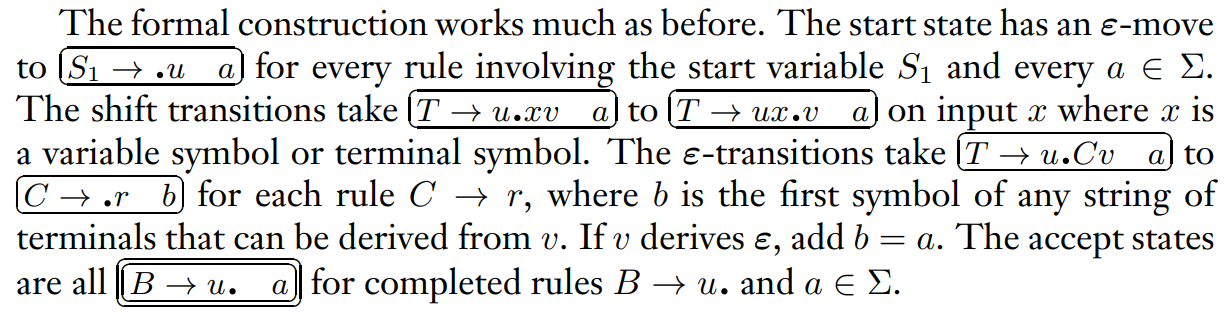
\includegraphics[width=\linewidth]{DK1 formal specification.png}
    \caption{formal construction of \(K_{1}\) automaton from book \cite{sipser}, Part 1, chapter 2.4.}
    \label{figure 2}
\end{figure}

\vspace{15pt}

To convert \(K_{1}\) into \(DK_{1}\) using power-set construction is memory inefficient. Thus, instead of using power-set construction, we use subset construction where we construct only the reachable states. The reader can check the subset construction method here \cite{DFA}.\\

In \( DK_{1} \) automaton, a state encapsulates \(items\) (also referred to as \(dotted rules\)). Each \(item\) contains a production rule, a dot at the corresponding point in the rule to signify progress, and lookahead symbols. If this terminology is unfamiliar to you, please refer to the book "Introduction to the Theory of Computation”, part 1, chapter 2.4 \cite{sipser}.\\

% ----- Image: Example of DK_1 automaton
\begin{figure}[h!]
    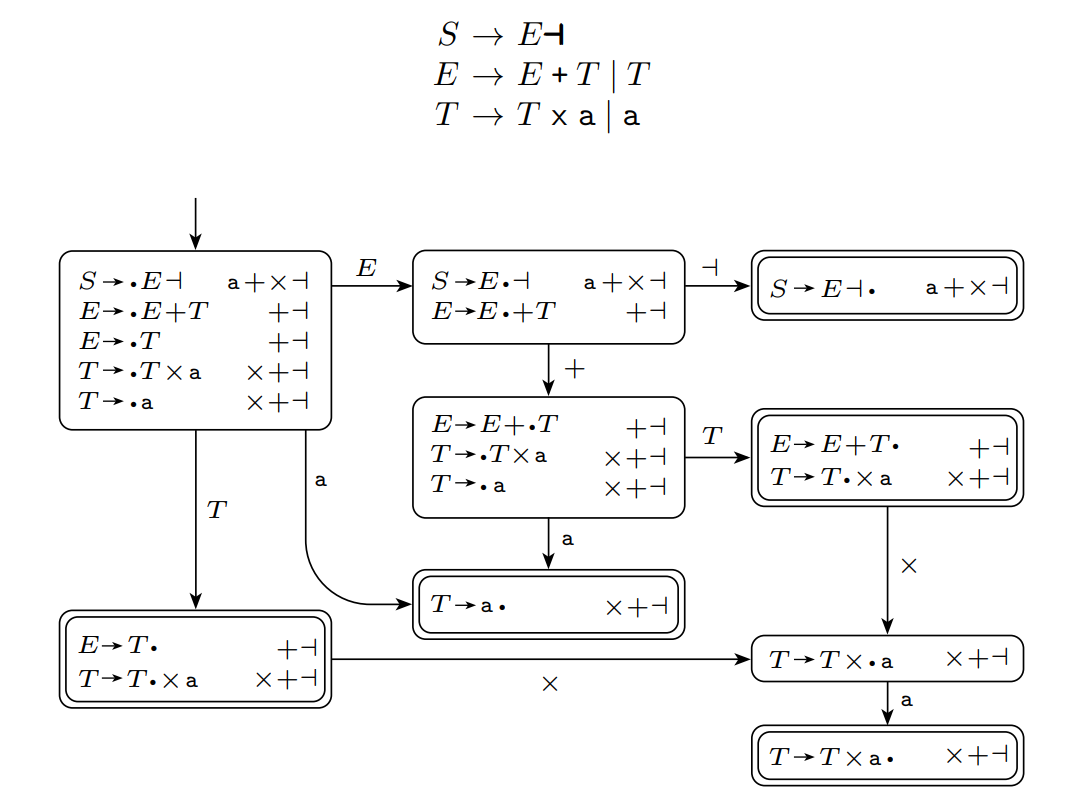
\includegraphics[width=\linewidth]{DK1 example.png}
    \caption{Example of \(DK_{1}\) Automaton. Image from book \cite{sipser}, part 1, chapter 2.4.}
    \label{figure 3}
\end{figure}

Based on the \( DK_{1} \) automaton specification from "Introduction to the Theory of Computation”, and the definition of finite deterministic automaton we aim to replicate the \( DK_{1} \) automaton's structure to align our implementation with the mathematical theory developed by Michael Sipser \cite{sipser}.\\

We create the following three classes:
\begin{enumerate}
    \item Class \(\boldsymbol{Item}\): \textit{The Items (dotted rules) serve as fundamental elements of the states in \( DK_{1} \). Therefore, we need a class to encapsulate this concept.}
    \item Class \(\boldsymbol{State}\): \textit{The need for a \(\boldsymbol{State}\) class is evident. An automaton consists of states, and each state encompasses several \(\boldsymbol{Item}\) objects.}
    \item Class \(\boldsymbol{DK_{1}}\): \textit{This class represents the entire \( DK_{1} \) automaton.}
\end{enumerate}

These classes will be grouped under a package named \(\boldsymbol{dk}\) - \href{https://github.com/fyfsb/dcfg/tree/main/src/main/java/dk}{GitHub/dk}.\\

Let’s delve into the details of each of these classes.

% Item Class
\subsection{Item Class}

The \(\boldsymbol{Item}\) class encapsulates the concept of an item (dotted rule) as presented in the book. It comprises a production rule, the location of a dot within this production rule, and lookahead symbols. To efficiently represent this concept, we will utilize three attributes along with several straightforward methods.\\

\textbf{Attributes:}
\begin{itemize}
    \item \(\boldsymbol{production}\): \textit{A \(\boldsymbol{Production}\) object that represents the production rule for this item.}
    \item \(\boldsymbol{dotIndex}\): \textit{An Integer that represents the location of the corresponding dot in the item}
    \item \(\boldsymbol{lookaheads}\): \textit{A set of \(\boldsymbol{Symbol}\) objects to represent all the lookahead symbols for this item}
\end{itemize}

\textbf{Methods:}
\begin{itemize}
    \item \(\boldsymbol{constructor}\): \textit{Initializes an \(\boldsymbol{Item}\) object with the specified production, dotIndex, and lookaheads.}
    \item \(\boldsymbol{isComplete}\): \textit{Returns true if the \(item\) is complete, i.e., if the dot is at the end of the production rule; otherwise, it returns false.}
    \item \(\boldsymbol{currentSymbol}\): \textit{Returns the symbol next to the dot in the production rule if it exists; Otherwise returns \(null\).}
    \item \(\boldsymbol{nextSymbol}\): \textit{Returns the symbol after the symbol next to the dot in the production rule if it exists, Otherwise returns \(null\). These methods, are trivial but shorten the whole implementation code significantly.}
    \item \(\boldsymbol{equals}\): \textit{Determines if two \(\boldsymbol{Item}\) objects are equal in all attributes: production, dotIndex, and lookaheads.}
    \item \(\boldsymbol{hashCode}\): \textit{Returns a hash code of the item.}
    \item \(\boldsymbol{sameProductionAndDot}\): \textit{This method is similar to \(\boldsymbol{equals}\), but it doesn't compare lookaheads. During the lookahead calculation, it's essential to identify identical production rules and dotIndex for grouping the lookaheads.}
    \item \(\boldsymbol{addLookaheads}\): \textit{Merges two sets of lookahead symbols}
\end{itemize}

\begin{codeblock}[Item Class. Java implementation on \href{https://github.com/fyfsb/dcfg/blob/main/src/main/java/dk/Item.java}{GitHub/Item}]
    class Item {
        Production production;
        int dotIndex;
        Set<Symbol> lookaheads;

        Item(Production production, int dotIndex, Set<Symbol> lookaheads) {}
        boolean isComplete() {}
        Symbol currentSymbol() {}
        Symbol nextSymbol(){}
        boolean equals(Object obj) {}
        int hashCode() {}
        boolean sameProductionAndDot(Item item) {}
        void addLookaheads(Set<Symbol> newLookaheads) {}
    }
\end{codeblock}

\vspace{10pt}

% State Class
\subsection{State Class}

The \(\boldsymbol{State}\) class represents a state within the \(DK_{1}\) automaton. It comprises a set of \(\boldsymbol{Item}\) objects, a local transition function specific to this state, and a set of complete rules, which are \(\boldsymbol{Item}\) objects with a dot at the end of the production rule.\\

\textbf{Attributes:}
\begin{itemize}
    \item \(\boldsymbol{items}\): \textit{A set of \(\boldsymbol{Item}\) objects that represents all the items for this state}
    \item \(\boldsymbol{transitionFunction}\): \textit{A Map\(<\)Symbol, State\(>\) representing the neighboring states of the current state. In other words, the \(\boldsymbol{transitionFunction}\) tracks paths from the current state to other states via a specific \(\boldsymbol{Symbol}\) object.}
    \item \(\boldsymbol{completeItems}\): \textit{A set of \(\boldsymbol{Item}\) objects to represent all the complete rules.}
\end{itemize}

\textbf{Methods:}
\begin{itemize}
    \item \(\boldsymbol{addItem}\): \textit{adds a new \(\boldsymbol{Item}\) object to the items. If a similar item with the same production and dotIndex already exists, the method simply merges the lookaheads and returns false.}
    \item \(\boldsymbol{sameItems}\): \textit{Returns true if two \(\boldsymbol{State}\) objects possess identical sets of \(\boldsymbol{Item}\) objects. Although two states may be identical, they might not be considered equal if one is still under construction and its \(\boldsymbol{transitionFunction}\) isn’t finalized. Therefore, identity is checked using the items.}
    \item \(\boldsymbol{createTransitionState}\): \textit{Creates and returns a new \(\boldsymbol{State}\) object with a given set of items. If the state with the same items already exists, the method doesn’t create a new state and returns an existing one. Creating new transition states is necessary in the construction process of the automaton.}
\end{itemize}

\begin{codeblock}[State Class.  Java implementation on \href{https://github.com/fyfsb/dcfg/blob/main/src/main/java/dk/State.java}{GitHub/State}]
    class State {
        Set<Item> items;
        Map<Symbol, State> transitionFunction;
        Set<Item> completeItems;

        boolean addItem(Item newItem) {}
        boolean sameItems(State newState) {}
        State createTransitionState(Set<Item> transitionItems, Set<State> states, Grammar g) {}
    }
\end{codeblock}

\vspace{10pt}

% DK1 Class
\subsection{DK1 Class}

The \(\boldsymbol{DK1}\) class represents the concept of the entire \(\boldsymbol{DK_{1}}\) deterministic finite automaton. Thus, it should encompass all the tuple elements mentioned in the definition of the DFA.\\

\textbf{Attributes:}
\begin{itemize}
    \item \(\boldsymbol{start}\): \textit{A \(\boldsymbol{start}\) object representing the start state of the automaton.}
    \item \(\boldsymbol{states}\): \textit{A set of \(\boldsymbol{start}\) objects representing all the states of the automaton.}
    \item \(\boldsymbol{grammar}\): \textit{A \(\boldsymbol{Grammar}\) object representing the input CFG.}
\end{itemize}

Let's ensure these three attributes encompass all elements of the DFA's 5-tuple.

\begin{enumerate}
    \item States (\(\boldsymbol{Q}\)):  \textit{\(\boldsymbol{DK1.states}\).}
    \item Alphabet (\(\boldsymbol{\Sigma}\)):  \textit{\(\boldsymbol{DK1.grammar.terminals}\) \(\cup\) \(\boldsymbol{DK1.grammar.nonterminals}\).}
    \item Transition Function (\(\boldsymbol{\delta}\)):  \textit{Since each \(\boldsymbol{State}\) object possesses its own local \(\boldsymbol{transitionFunction}\), \(\boldsymbol{\delta}\) is represented through \(\boldsymbol{DK1.states}\).}
    \item Start state (\(\boldsymbol{q_{0}}\)):  \textit{\(\boldsymbol{DK1.start}\).}
    \item Set of accept states (\(\boldsymbol{F}\)):  \textit{Following the literature \cite{sipser}, a state is considered accepting if it contains a completed rule, specifically, an item with a dot at the end. Consequently, we can identify accepting states by iterating through the items of a \(\boldsymbol{State}\) and using the \(\boldsymbol{Item.isComplete()}\) method. \(\boldsymbol{DK1.states}\).}
\end{enumerate}

All the methods mentioned below are quite complex from the implementation point of view. Here, we'll provide a brief description and reserve a detailed specification for the subsequent sections.\\

\textbf{Methods:}
\begin{itemize}
    \item \(\boldsymbol{constructor}\): \textit{Constructs an entire \(DK_{1}\) automaton based on the provided input \(\boldsymbol{Grammar}\) object.}
    \item \(\boldsymbol{dk1Test}\): \textit{Returns true if the \(\boldsymbol{Grammar}\) is LR(1), false otherwise.}
    \item \(\boldsymbol{parseString}\): \textit{Returns a derivation tree for the given \textbf{valid string}.}
    \item \(\boldsymbol{findHandle}\): \textit{Returns the handle for the given \textbf{valid string}.}
    \item \(\boldsymbol{makeReduction}\): \textit{Makes a one-step reduction of the \textbf{valid string} based on the provided handle.}
\end{itemize}

\begin{codeblock}[DK1 Class. Java implementation on \href{https://github.com/fyfsb/dcfg/blob/main/src/main/java/dk/DK1.java}{GitHub/DK1}]
    class DK1 {
        State start;
        Set<State> states;
        Grammar g;

        DK1(Grammar grammar) {}
        boolean dk1Test() {}
        DTE parseString(String validString) {}
        Item findHandle(List<Symbol> validStringArray) {}
        List<Symbol> makeReduction(List<Symbol> validStringArray, Item handle) {}
    }
\end{codeblock}

\newpage


% DK1 Automaton Builder for a CFG
\section{\(DK_{1}\) Automaton Builder for a CFG}\label{sec:DK1 Automaton Builder for a CFG}

We have built a solid framework to construct the \(DK_{1}\) automaton of a particular CFG. \(DK_{1}\) is a deterministic finite automaton that will help us to test the input grammar and then parse the source code. The implementation will closely follow the theory developed in the "Introduction to the Theory of Computation" \cite{sipser}. Note that the implementation process is intricate. For instance, while the example of the \(DK_{1}\) automaton for a basic grammar in \hyperref[figure 3]{Figure 2.2} has only 9 states with a few items, the \(DK_{1}\) of the C0 grammar comprises 3264 states with a vast number of items. Even a small error in the implementation can drastically alter the automaton.

\vspace{10pt}

% DK1.constructor
\subsection{DK1.constructor}

Parameters: \textit{Grammar \(\boldsymbol{grammar}\).}

Returns: \textit{\(\boldsymbol{DK1}\).}\\

Java implementation on \href{https://github.com/fyfsb/dcfg/blob/main/src/main/java/dk/DK1.java}{GitHub/DK1}\\

\textbf{Specification:} \textit{Creates the \(DK_{1}\) automaton for the given CFG.}\\

The constructor method of the \(DK_{1}\) class creates the entire automaton. As previously emphasized, this is a delicate process. We will thus utilize several auxiliary methods to break down the intricate procedure into more manageable tasks.\\

% Start State Creation
\textbf{\textit{Start State Creation}}\\

Firstly, we need to initialize \(\boldsymbol{DK1.start}\), which encompasses all items where the left-hand attribute of the production is equal to \(\boldsymbol{Grammar.start}\). Additionally, \(\boldsymbol{DK1.lookaheads}\) should be set to \(\boldsymbol{Grammar.terminals}\), and \(\boldsymbol{DK1.dotIndex}\) should be assigned to the value 0.\\

Whenever a new state is created, it must be updated with \(\varepsilon\)-transitions as described in formal construction of \({K_{1}}\) Automaton. However, this updating process can be recursive. To address this, we introduce a specialized method \(\boldsymbol{makeEpsilonMoves}\). This method is responsible for updating the current state with \(\varepsilon\)-transitions until no further \(\varepsilon\)-transitions are possible for this state. The implementation details of this method are discussed in the next subsection.\\

\vspace{15pt}

% Make a Queue
\textbf{\textit{Make a Queue}}\\

Next, we create a queue structure, referred to as \(queue\), composed of \(\boldsymbol{State}\) objects. We use breadth-first search (BFS) to produce new neighboring states and to construct the entire automaton. The queue's first element is predictably \(\boldsymbol{DK1.start}\).\\

\vspace{15pt}

% Process the Queue
\textbf{\textit{Process the Queue}}\\

During each iteration, we extract and eliminate the first \(\boldsymbol{State}\) element from the queue, referred to as \(\boldsymbol{currentState}\). To generate new neighboring states, we must execute shift transitions as defined in formal construction of \({K_{1}}\) automaton. A separate method, \(\boldsymbol{makeShiftMoves}\), is defined to update the \(\boldsymbol{currentState}\) considering shift transitions. This method fills \(\boldsymbol{currentState.transitionFunction}\) completely with the appropriate transition paths.\\

To update the queue, we loop through \(\boldsymbol{currentState.transitionFunction}\), appending its neighboring states to the queue. However, to avoid infinite loops, we must never add a state to the queue more than once. We maintain a list of previously visited states, \(\boldsymbol{queueCheck}\), and use \(\boldsymbol{State.sameItems}\) to determine whether a state has been visited. If a neighbor state hasn't been visited, it will be added to the queue.\\

The end of this loop will complete the \(DK_{1}\) automaton building process. Now, let's detail the methods we used above: \(\boldsymbol{makeEpsilonMoves}\) and \(\boldsymbol{makeShiftMoves}\).

\vspace{20pt}

% makeEpsilonMoves
\subsection{makeEpsilonMoves}

Parameters: \textit{Grammar \(\boldsymbol{grammar}\).}

Returns: \textit{\(\boldsymbol{void}\).}\\

\textbf{Specification:} \textit{Implements the \(\varepsilon\)-transitions making process as described in the formal construction of the \({K_{1}}\) automaton.}\\

In simpler terms, if a state has an item with the dot following a nonterminal symbol, we must include all new items in the state, with this nonterminal as the left attribute of the production, dotIndex set to 0, and lookaheads updated as previously specified. The \(\boldsymbol{grammar}\) input parameter grants access to terminals, nonterminals, and productions.\\

Notably, this is a recursive operation. We use a while loop that continues as long as new items are added to the state. Within this loop, we cycle through items, attempting to introduce new items. The currently iterated item is labeled  \(\boldsymbol{currentItem}\). If the dot of \(\boldsymbol{currentItem}\) follows a nonterminal, we add a new item with the left set to this nonterminal, dotIndex to 0, and lookaheads are updated according to the book's specification. A method, \(\boldsymbol{lookaheadsFromSymbol}\), returns an updated set of lookahead symbols. Then, we iterate through all the \(\boldsymbol{Grammar.productions}\), selecting all productions with this nonterminal on the left, and creating a new item with the corresponding attributes. If a new item is added to the state during this iteration, the process repeats.\\

\begin{codeblock}[makeEpsilonMoves pseudocode. Java implementation on \href{https://github.com/fyfsb/dcfg/blob/main/src/main/java/dk/State.java}{GitHub/State}]
    Function makeEpsilonMoves
    Input: Grammar g
    Output: void

    Initialize a flag 'newItems' to false

    Repeat
    Set 'newItems' to false

    // Create a copy of items to avoid ConcurrentModificationException
    For each 'currentItem' in a copy of 'items' set
    Get 'currentSymbol' from 'currentItem'
    If 'currentSymbol' is null, skip to the next iteration

    If 'currentSymbol' is not a terminal symbol
    Get 'nextSymbol' from 'currentItem'

    // Determine lookaheads
    Declare 'lookaheads' set
    If 'nextSymbol' is null
    Copy 'currentItem's lookaheads to 'lookaheads'
    Else
    Calculate 'lookaheads' using 'nextSymbol' and grammar 'g'

    For each 'production' in grammar 'g'
    If the left side of 'production' equals 'currentSymbol'
    Create a new item 'newItem' with 'production', position 0, and 'lookaheads'
    Update 'newItems' flag if 'newItem' is successfully added to items set
    Until 'newItems' is false
\end{codeblock}

\vspace{30pt}

% lookaheadsFromSymbol
\subsection{lookaheadsFromSymbol}

Parameters: \textit{Symbol \(\boldsymbol{symbol}\), Set\(<\)Symbol\(>\) \(\boldsymbol{symbols}\), Grammar \(\boldsymbol{grammar}\).}

Returns: \textit{Set\(<\)Symbol\(>\) \(\boldsymbol{lookaheadsFromSymbol}\) .}\\

\textbf{Specification:} \textit{Calculates and returns all the terminal symbols that can be the first symbol of the valid strings, derivable from the given \(\boldsymbol{symbol}\) within this \(\boldsymbol{grammar}\). As this method is also recursive, the \(\boldsymbol{symbols}\) input parameter keeps track of visited symbols to avoid infinite loops.}\\

\begin{codeblock}[lookaheadsFromSymbol pseudocode. Java implementation on \href{https://github.com/fyfsb/dcfg/blob/main/src/main/java/dk/State.java}{GitHub/State}]
    Function lookaheadsFromSymbol
    Input: Symbol symbol, Set of Symbols symbols, Grammar g
    Output: Set of terminal Symbols that can be the first symbol of derivable strings from 'symbol'

    Initialize an empty set of Symbols 'lookaheads'
    Add 'symbol' to the set 'symbols'

    // If the symbol is terminal, return a set containing only this symbol
    If 'symbol' is a terminal symbol
    Add 'symbol' to 'lookaheads'
    Return 'lookaheads'
    Else
    For each 'production' in the productions of grammar 'g'
    If the left side of 'production' equals 'symbol'
    Get the first Symbol 'derivedSymbol' from the right side of 'production'
    // Recursively compute lookaheads if derivedSymbol has not been visited
    If 'derivedSymbol' is not in 'symbols'
    Add all elements from the result of lookaheadsFromSymbol(derivedSymbol, symbols, g) to 'lookaheads'

    Return 'lookaheads'
\end{codeblock}

\vspace{30pt}

% makeShiftMoves
\subsection{makeShiftMoves}

Parameters: \textit{Set\(<\)State\(>\) \(\boldsymbol{states}\), Grammar \(\boldsymbol{grammar}\).}

Returns: \textit{\(\boldsymbol{void}\).}\\

\textbf{Specification:} \textit{Implements the shift transitions making process specified in the formal construction of the \({K_{1}}\) automaton. This method initializes new states, when necessary. The \(\boldsymbol{states}\) input parameter ensures not to create the same state multiple times.}\\

The core task of this method is advancing the dot by one symbol to the right. This action triggers new paths/transitions for the automaton. However, the neighboring state might not have been established. Hence, we determine new pathways and, if the requisite state is absent, employ the \(\boldsymbol{State.createTransitionState(...)}\) method to initialize the neighbor.\\

\begin{codeblock}[makeShiftMoves pseudocode. Java implementation on \href{https://github.com/fyfsb/dcfg/blob/main/src/main/java/dk/State.java}{GitHub/State}]
    Function makeShiftMoves
    Input: Set of States states, Grammar g
    Output: void

    Initialize a map 'symbolToItemsMap' to map Symbols to Sets of Items

    // Mapping transition symbols to their respective items
    For each 'item' in 'items'
    Get 'currentSymbol' from 'item'
    If 'currentSymbol' is null, continue to the next iteration

    Add 'item' to the set in 'symbolToItemsMap' corresponding to 'currentSymbol'

    // Creating transition paths
    For each entry in 'symbolToItemsMap'
    Get 'transitionSymbol' and Set of Items 'transitionItems' from the entry
    Create a State 'transitionState' for 'transitionItems' using states and grammar 'g'
    Map 'transitionSymbol' to 'transitionState' in 'transitionFunction'
\end{codeblock}

\newpage


% DK1 Test
\section{\(DK_{1}\) Test}\label{sec:DK1 Test}

Having already constructed the \(DK_{1}\) automaton for the input grammar, we are ready to test whether our grammar belongs to LR(1), or not. For this purpose, we will instantiate the method \(\boldsymbol{dk1Test}\) within the \(\boldsymbol{DK1}\) class.\\

The book \cite{sipser}, part 1, chapter 2.4, Parsing and LR(K) Grammars, provides the following formal specification of the \(DK_{1}\) Test:

% Image of formal specification of DK1 test

\begin{figure}[h!]
    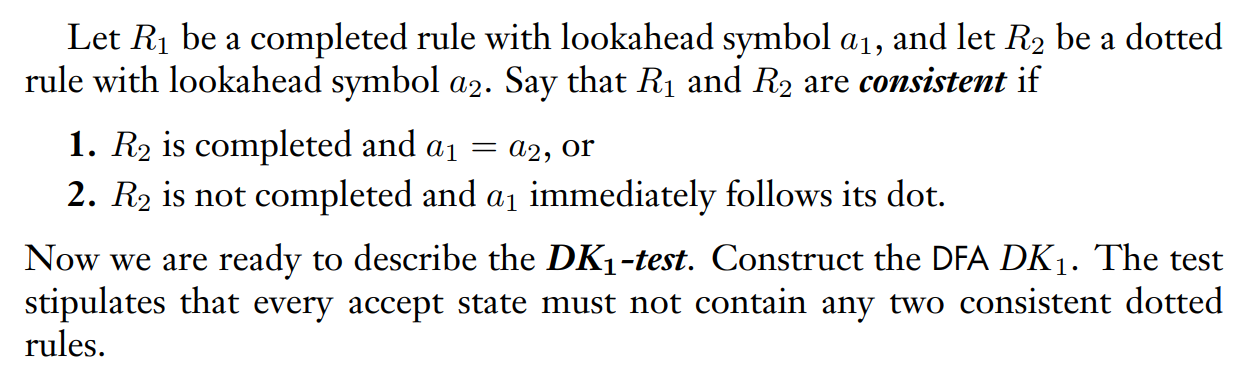
\includegraphics[width=\linewidth]{DK1 test conditions.png}
    \caption{\(DK_{1}\) test specification from book \cite{sipser}, part 1, chapter 2.4.}
    \label{figure 4}
\end{figure}


\vspace{15pt}

% dk1Test
\subsection{DK1Test}

The method \(\boldsymbol{DK1Test}\) iterates through all the states in \(\boldsymbol{DK1.states}\), with the current state referred to as \(\boldsymbol{currentState}\). Within this, another loop iterates over the complete rule items inside \(\boldsymbol{currentState}\), which we will label as \(\boldsymbol{R1}\). Furthermore, another loop iterates through items other than \(\boldsymbol{R1}\), which we designate as \(\boldsymbol{R2}\).\\

Following this, we encounter two cases:
\begin{itemize}
    \item \(\boldsymbol{R2}\) represents a complete rule:
\end{itemize}

We examine if \(\boldsymbol{R1.lookaheads}\) and \(\boldsymbol{R2.lookaheads}\) share a common \(\boldsymbol{Symbol}\) object. If they do, the \(DK_{1}\) Test fails due to condition 1 specified in the book.

\begin{itemize}
    \item \(\boldsymbol{R2}\) isn't a complete rule:
\end{itemize}

We determine if \(\boldsymbol{R1.lookaheads}\) contain \(\boldsymbol{R2.currentSymbol()}\) (the symbol positioned after the dot). If this is the case, the \(DK_{1}\) Test fails because of condition 2 as specified in the book.\\

If all the states pass these checks, then the \(DK_{1}\) Test is deemed successful!\\

\begin{codeblock}[DK1Test pseudocode. Java implementation on \href{https://github.com/fyfsb/dcfg/blob/main/src/main/java/dk/DK1.java}{GitHub/DK1}]
    Function DK1Test
    Input:
    Output: Returns true if the Grammar is LR(1), false otherwise

    For each 'currentState' in 'states'
    For each 'R1' in the items of 'currentState'
    For each 'R2' in the items of 'currentState'
    If 'R1' is not complete, break the innermost loop
    If 'R1' equals 'R2', continue to the next iteration of the innermost loop

    If 'R2' is complete
    For each 'symbol' in the lookaheads of 'R1'
    If the lookaheads of 'R2' contains 'symbol'
    Log "Failing State DK1_Test_Failing_Condition_1" with details of 'R1', 'R2', and 'currentState'
    Return false
    Else
    Get 'currentSymbol' from 'R2'
    If the lookaheads of 'R1' contains 'currentSymbol'
    Log "Failing State DK1_Test_Failing_Condition_2" with details of 'R1', 'R2', and 'currentState'
    Return false

    Return true
\end{codeblock}

\newpage


% Analysis and Corrections of C0 Grammar based on DK1 Test
\section{Analysis and Corrections of C0 Grammar based on \(DK_{1}\) Test}\label{sec:Analysis and Corrections of C0 Grammar based on DK1 Test}

Regrettably, the initial C0 grammar (as shown in \hyperref[fig:grammar_c0]{Figure 1.1}) doesn’t pass the \(DK1\) Test without a few production rule adjustments.\\

The essential causes of failure are:

\begin{enumerate}
    % 1
    \item A singular lookahead symbol fails to definitively discern between multiplication and pointer dereference symbols \(\ast\). This became evident through the failure triggered by \({DK_{1}}\) Test failure condition 2 in one of the states of the C0's \(DK1\) automaton with these items:
    \begin{verbatim}
    R1:     <F> → <id>.      lookaheads:   ||  &&  -  +  /  *  )
    R2:     <id> → <id>.*    lookaheads:   ||  &&  -  +  /  *  )  [  &  .
    \end{verbatim}
    Solution: \\
    The asterisk symbol \(\ast\) is adjusted to \(\textquotesingle\) for the pointer dereference. Consequently, the modified production is:
    \begin{verbatim}
    <id> → <id>'
    \end{verbatim}
    In the next section, we will withdraw this change by using the pre-processor.

    % 2
    \item In three production rules the recursion direction has to be adjusted.
    The test failed by \({DK_{1}}\) Test failure condition 2 at the below state:
    \begin{verbatim}
    R1:     <VaDS> → <VaD>.           lookaheads:   ;
    R2:     <VaDS> → <VaD>.;<VaDS>    lookaheads:   ;
    \end{verbatim}
    The explanation is that, with the current single lookahead, it’s challenging to conclusively decide on the suitable reduction:
    \begin{verbatim}
    <VaDS> ← <VaD>  or  <VaDS> ← <VaD>;<VaDS>
    \end{verbatim}

    Solution: \\
    Invert the direction of the recursion for clarity. Instead of the initial production:
    \begin{verbatim}
    <VaDS> → <VaD>|<VaD>;<VaDS>
    \end{verbatim}
    the revised version is:
    \begin{verbatim}
    <VaDS> → <VaD>|<VaDS>;<VaD>
    \end{verbatim}

    The same adjustment is applied to analogous recursive productions \texttt{<TyDS>}, and \texttt{<StS>}, leading to:
    \begin{verbatim}
    <TyDS> → <TyD> | <TyDS>;<TyD>
    <StS> → <St> | <StS>;<St>
    \end{verbatim}

    %3
    \item Type ambiguity between Boolean and Arithmetic variables.

    There’s a failure by \({DK_{1}}\) Test failure condition 2 in one of the states of the C0's \(DK1\) automaton with these items:
    \begin{verbatim}
    R1:		<F> → <id>.   lookaheads:   <=  ==  /  >=  > -  < !=  +  *  )
    R2:		<BF> → <id>.  lookaheads:   ||   &&  )
    \end{verbatim}
    The explanation of the test failure is that, without prior variable type information, deciding on the appropriate reduction, whether
    \begin{verbatim}
     <F> ← <id>  or  <BF> ← <id>,
    \end{verbatim}
    is nondeterministic.\\

    Solution: \\
    Implement a distinction in the variable type by replacing the production rule
    \begin{verbatim}
    <BF> → <id>  with  <BF> →(bool)<id>
    \end{verbatim}

    In the next section, we will also discuss how to withdraw this change using the pre-processor.\\

    After these adjustments, the grammar is successfully classified as LR(1). Additionally, note that the simultaneous use of \(-\) symbol for unary and binary minus doesn’t introduce ambiguity to the grammar. However, we will need to distinguish between those two, in order to differentiate multiplication and pointer dereferencing during the pre-processing phase.
\end{enumerate}

% updated grammar image

\newpage


% Pre-processing for C0 Source Code
\section{Pre-processing for C0 Source Code}\label{sec:Pre-processing for C0 Source Code}

A pre-processor is a tool that processes the source code before the actual compilation begins. We plan to specify a basic pre-processor to manage extra whitespaces, tabs, and end-lines in the source code. Creating an in-depth pre-processor is beyond the scope of this thesis. The asterisk symbol \(\ast\) introduced ambiguity in our grammar. However, languages like C++ allow programmers to use it for dereferencing. We will discuss how the pre-processor can address this, allowing programmers to use the symbol seamlessly. Similarly, we'll discuss how to remove the additional \texttt{(bool)} prefix before \texttt{<id>} that identifies a Boolean factor.

\vspace{10pt}

% eliminateExtraWhiteSpace
\subsection{eliminateExtraWhiteSpace}

Parameters: \textit{List\(<\)Symbol\(>\) \(\boldsymbol{validStringArray}\).}

Returns: \textit{List\(<\)Symbol\(>\) \(\boldsymbol{updatedValidStringArray}\).}\\

Java implementation on \href{https://github.com/fyfsb/dcfg/blob/main/src/main/java/grammar/Grammar.java}{GitHub/Grammar}\\

\textbf{Specification:} \textit{The method removes excess whitespace from the provided \(\boldsymbol{validStringArray}\) as detailed below}\\

\begin{enumerate}
    \item If there are adjacent whitespaces, remove them, and leave only one.
    \item Erase all the tabs and end-lines: \texttt{\textbackslash  t} \texttt{\textbackslash  n}
    \item Erase all surrounding whitespace of these symbols:
    \begin{verbatim}
        ,    ;    +    -    *    /    &    |    !    =
    \end{verbatim}
\end{enumerate}

This method offers programmers some flexibility when using whitespaces. Further refinement of this method would necessitate careful implementation and rigorous testing. Therefore, we'll pause here and resume the primary focus of this thesis.

\vspace{30pt}

% Distinguish multiplication and pointer dereferencing
\subsection{Distinguish multiplication and pointer dereferencing}

In the updated C0 grammar we use \(\textquotesingle\) instead of \(\ast\) when dereferencing a pointer. By distinguishing between these two cases in the pre-processing phase, we can allow programmers to use \(\ast\) for pointer dereferencing, even though the grammar uses \(\textquotesingle\). Once we identify the asterisks used for pointer dereferencing, we'll replace them with \(\textquotesingle\) before the parsing process starts.\\

To differentiate between multiplication and pointer dereferencing, we need to observe the immediate symbol to the right of the \(\ast\).

\begin{verbatim}
    <id> → <id>*
    <T> → <T>*<F>
\end{verbatim}

To differentiate between the two, we'll compare the potential first terminals of \texttt{<F>} and those that can stand immediately to the right of \texttt{<id>}.\\

The first terminal of \texttt{<F>} can be:
\begin{center}
    \begin{tabular}{|c|c|c|c|}
        \hline
        A letter derivable from \( <Le> \) & Unary \( - \) & \( ( \) & A digit derivable from \( <Di> \) \\
        \hline
    \end{tabular}
\end{center}

The first terminal standing to the right of \texttt{<id>} can be:
\begin{center}
    \begin{tabular}{|c|c|c|c|c|c|c|c|}
        \hline
        \( . \) & \( [ \) & \( \ast \) & \( \& \) & \( = \) & \( / \) & \( + \) & Binary \( - \)\\
        \hline
        \( > \) & \( < \) & \( \! \) & \( ; \) & \( \} \) & \( , \) & Whitespace & \\
        \hline
    \end{tabular}
\end{center}

Notably, the minus symbol is the obly overlapping element between the two lists. However, it represents a unary operation in the first context and a binary one in the second. Therefore, to correctly identify the pointer dereference symbol, we must differentiate between the unary and binary minus operations within the C0 grammar.\\

To do so, we should observe what can be on the left of the \(-\) symbol.\\

On the left of Binary \(-\) can be:
\begin{center}
    \begin{tabular}{|c|c|c|c|c|c|c|}
        \hline
        \( ) \) & \( <C> \) & \( <Na> \) & \( ] \) & \( ' \) & \( \& \)\\
        \hline
    \end{tabular}
\end{center}

On the left of Unary \(-\) can be:
\begin{center}
    \begin{tabular}{|c|c|c|c|c|c|c|c|c|c|c|c|}
        \hline
        \( \ast \) & \( / \) & \( + \) & \( - \) & \( > \) & \( = \) & \( < \) & \( \&\& \) & \( || \) & \( \) & \( , \) & \( ( \)\\
        \hline
    \end{tabular}
\end{center}

Thus we know how to differentiate between binary and unary minus. Consequently, we also know how to distinguish between multiplication and pointer dereferencing.\\

During the pre-processing phase, when encountering \(\ast\), we'll inspect the subsequent symbol. If it is a letter, unary minus, an opening bracket, or a digit, we'll replace it with \(\textquotesingle\). Otherwise, we leave it as it is.

\vspace{30pt}

% Distinguish arithmetic and boolean identifiers
\subsection{Distinguish arithmetic and boolean identifiers}

In this final segment of our pre-processing discussion, we aim to differentiate between boolean and arithmetic identifiers, and address the redundant \texttt{(bool)} prefix in the modified production:

\begin{verbatim}
    <BF> →(bool)<id>.
\end{verbatim}

To distinguish between boolean and arithmetic identifiers, understanding whether a variable is global or local is essential. We should create a set containing boolean variable names, initializing it with global variables from \texttt{<VaDS>} and subsequently updating it with local variables at the start and end of the method.

\newpage


% Derivation Tree Structure and Implementation
\section{Derivation Tree Structure and Implementation}\label{sec:Derivation Tree Structure and Implementation}

At this point, we have prepared all the tools in order to start the parsing process. But, just parsing is not enough if we do not store its result. That’s why we need to build a structure called a derivation tree that will help us to conveniently store and afterward efficiently use the data provided during the parsing phase. When the parsing process is complete, we will hand over the parse tree of the given source code to our college Irakli Khotchava who will use it to generate relevant assembly code.

\vspace{10pt}

% Derivation tree structure
\subsection{Derivation tree structure}

We take the derivation tree structure from the book "System Architecture: An Ordinary Engineering Discipline" \cite{sysbook}, chapter 10.1.

\begin{definition}[3.0]
    A derivation tree element is defined as a 4-tuple \((label, father, fson, bro)\), where
    \begin{enumerate}
        \item \(label\) is a string, the actual content of this element,
        \item \(father\) represents the parent of this element in the derivation tree. If the element is the \(root\) we make \(father\) = \(null\),
        \item \(fson\) is the first son (leftmost) of this element in the derivation tree. If the element is a \(leaf\) we make \(fson\) = \(null\),
        \item \(bro\) represents the right brother of the current element in the derivation tree if there is such a brother. Otherwise we make \(bro\) = \(null\).
    \end{enumerate}

    A derivation tree is a tree derived from the root derivation tree element.

\end{definition}
\setlength{\parindent}{0pt}

\vspace{10pt}

% Derivation tree structure implementation
\subsection{Derivation tree structure implementation}

To replicate the structure given above, we will create the class \(\boldsymbol{DTE}\) under a package named \(\boldsymbol{tree}\). \(\boldsymbol{DTE}\) will encapsulate the concept of derivation tree element.\\

\textbf{Attributes:}
\begin{itemize}
    \item \(\boldsymbol{label}\): \textit{A \(\boldsymbol{Symbol}\) object representing the label string of the element. Since, our goal is for each tree element to contain only one terminal or nonterminal symbol, the type of \(\boldsymbol{label}\) is \(\boldsymbol{Symbol}\).}
    \item \(\boldsymbol{fatehr}\): \textit{A \(\boldsymbol{DTE}\) object representing the father.}
    \item \(\boldsymbol{fson}\): \textit{A \(\boldsymbol{DTE}\) object representing the fson.}
    \item \(\boldsymbol{bro}\): \textit{A \(\boldsymbol{DTE}\) object representing the bro.}
\end{itemize}

\(\boldsymbol{DTE}\) class has several methods necessary for the code generation process, but for the derivation tree building, we use only one method called \(\boldsymbol{updateTheParseTree}\) that will update the current derivation tree on every reduction step during the parsing process and finally return the entire derivation tree of the given source code.

\vspace{10pt}

% updateTheParseTree
\subsection{Static updateTheParseTree}

Parameters: \textit{List\(<\)DTE\(>\) \(\boldsymbol{parseTree}\), Item \(\boldsymbol{handle}\).}

Returns: \textit{List\(<\)DTE\(>\) \(\boldsymbol{updatedParseTree}\)}\\

\textbf{Specification:} \textit{updates the current \(\boldsymbol{parseTree}\) with respect to the given handle reduction step of the parsing process.}\\

At the beginning of the parsing process, we are given only the source code and we do not have any idea what the derivation tree will look like. At every step of the parsing process, we can find the forced handle and make one reduction step. Thus, we can not start building the derivation tree from the root, we have to start from the leaves and reverse engineer to the root. At the very first call of this method, the List \(\boldsymbol{parseTree}\) will contain a consistent sequence of leaves each of them containing one symbol from the tokenization of the source code. These leaves will not have \(fathers\), \(fsons\), nor \(bros\), all these values will be \(null\).\\

In a step of the reduction with the given handle, the method will:
\begin{enumerate}
    \item Fetch the new father’s label from \(\boldsymbol{handle.production.left}\) named \(\boldsymbol{fatherSymbol}\).
    \item Find the subsequence of the \(\boldsymbol{parseTree}\) that we will reduce to the \(\boldsymbol{fatherSymbol}\).
    \item \(\boldsymbol{rightIndex = handle.dotIndex}\), (where \(\boldsymbol{handle.dotIndex}\) follows the last symbol of the reduction string)
    \item \(\boldsymbol{leftIndex = rightIndex - handle.production.right.size()}\).
    \item Set up brotherhood inside this subsequence. Start from \(\boldsymbol{leftIndex}\) and make the next right element of the \(\boldsymbol{parseTree}\) its brother till \(\boldsymbol{rightIndex}\).
    \item Create the father \(\boldsymbol{DTE}\) object \(\boldsymbol{father}\) with:
    \begin{itemize}
        \item \(\boldsymbol{label = fatherSymbol}\),
        \item \(\boldsymbol{fson = parseTree.get(leftIndex)}\),
    \end{itemize}
    \item Set \(\boldsymbol{father}\) as the father of the derivation tree elements from \(\boldsymbol{leftIndex}\) to \(\boldsymbol{rightIndex}\).
    \item Erase the \(\boldsymbol{leftIndex}\) to \(\boldsymbol{rightIndex}\) segment of \(\boldsymbol{parseTree}\) and replace it with \(\boldsymbol{father}\).
    \item Return the updated \(\boldsymbol{parseTree}\).
\end{enumerate}

\vspace{10pt}

\begin{codeblock}[updateTheParseTree pseudocode. Java implementation on \href{https://github.com/fyfsb/dcfg/blob/main/src/main/java/tree/DTE.java}{GitHub/DTE}]
    Function updateTheParseTree
    Input: ArrayList of DTEs 'parseTree', Item 'handle'
    Output: Updated ArrayList of DTEs

    Get 'parentSymbol' from the left side of the production of 'handle'
    Calculate 'rightIndex' as the dot index of 'handle'
    Calculate 'leftIndex' as 'rightIndex' minus the size of the right side of the production of 'handle'

    // Make Brothers
    For i from 'leftIndex' to 'rightIndex' - 1
    Set the brother of the DTE at index i in 'parseTree' to the DTE at index i + 1

    // Create father and make connection
    Create a new DTE 'father' with 'parentSymbol'
    Set the first son of 'father' to the DTE at 'leftIndex' in 'parseTree'
    For i from 'leftIndex' to 'rightIndex'
    Set the father of the DTE at index i in 'parseTree' to 'father'

    // Erase Children from the parse tree array and put father in their place
    Initialize a new ArrayList of DTEs 'newParseTree'
    Add all DTEs from 'parseTree' up to 'leftIndex' to 'newParseTree'
    Add 'father' to 'newParseTree'
    Add all DTEs from 'parseTree' starting from 'rightIndex' to 'newParseTree'

    Return 'newParseTree'
\end{codeblock}

\newpage


% Parsing and Derivation Tree Building
\section{Parsing and Derivation Tree Building}\label{sec:Parsing and Derivation Tree Building}

We have arrived at the culmination of this Chapter of the thesis paper. The most exciting part of the process is to parse the source code and in real life test that the foundation theory and the implementation are correct. In \hyperref[sec:Pre-processing for C0 Source Code]{Sect.2.7} we have already outlined the pre-processor. However, the \href{https://github.com/fyfsb/dcfg/}{GitHub} implementation of the pre-processor includes only the elimination of extra spaces. Therefore, after the tokenization of the source code, the pre-processor will eliminate all the extra whitespace, as detailed in \hyperref[sec:Pre-processing for C0 Source Code]{Sect.2.7}. Subsequently, the parsing process will begin, according to the modified C0 grammar as specified in \hyperref[sec:Analysis and Corrections of C0 Grammar based on DK1 Test]{Sect.2.6}.  \\

If you carefully read the book \cite{sipser}, chapter 2.4, you will notice that the \(DK_{1}\) is the parsing tool for our CFG. The \(DK_{1}\) automaton identifies the handles of the given valid string. If we know the handle of the valid string, we know the reduction step and we will reduce the valid string until we get to the start symbol of the given CFG.\\

For parsing we implement three methods inside the class \(\boldsymbol{DK1}\):  \(\boldsymbol{findHandle}\), \(\boldsymbol{makeReduction}\), and \(\boldsymbol{parseValidString}\).

\vspace{10pt}

% findHandle
\subsection{findHandle}

Parameters: \textit{List\(<\)Symbol\(>\) \(\boldsymbol{validStringArray}\).}

Returns: \textit{Item \(\boldsymbol{handle}\)}\\

\textbf{Specification:} \textit{finds and returns the forced handle for the given \(\boldsymbol{validStringArray}\) using the current \(DK_{1}\) automaton.}\\

In order to find the handle for the given valid string we should traverse the \(DK_{1}\) automaton and at some point, we will arrive at the accepting state which will have the handle item representing the upcoming reduction rule.

% ----- Image: Corollary about finding the handle
\begin{figure}[h!]
    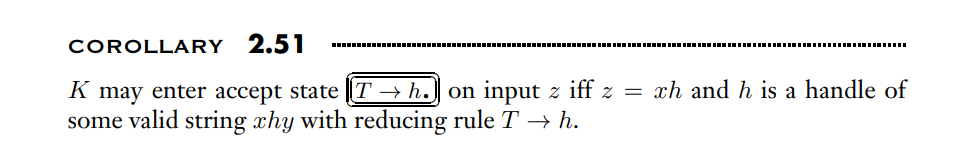
\includegraphics[width=\linewidth]{Identify Handle.png}
    \caption{Corollary 2.51 from book \cite{sipser}, part 1, chapter 2.4.}
    \label{figure 5}
\end{figure}

\vspace{10pt}

\begin{codeblock}[findHandle pseudocode. Java implementation on \href{https://github.com/fyfsb/dcfg/blob/main/src/main/java/dk/DK1.java}{GitHub/DK1}]
    Function findHandle
    Input: ArrayList of Symbols 'validStringArray'
    Output: Item representing the handle, or null if no handle is found

    Initialize 'currentState' to start state
    Initialize 'dotIndex' to 0
    Get 'currentSymbol' from 'validStringArray' at 'dotIndex'

    While 'currentState' is not null
    If 'currentState' has complete items
    Set 'lookahead' to the symbol at 'dotIndex' in 'validStringArray', or null if 'dotIndex' is out of bounds

    For each 'item' in the complete items of 'currentState'
    If 'lookahead' is not null and 'lookahead' is not in the lookaheads of 'item', continue to next iteration
    Return a new Item with the production of 'item', 'dotIndex', and an empty set of lookaheads

    // Make transition
    Initialize 'madeTransition' to false
    For each entry in the transition function of 'currentState'
    Get 'transitionSymbol' and 'transitionState' from the entry

    If 'transitionSymbol' equals 'currentSymbol'
    Increment 'dotIndex'
    Update 'currentState' to 'transitionState'
    Update 'currentSymbol' to the next symbol in 'validStringArray' or null if 'dotIndex' is out of bounds
    Set 'madeTransition' to true and break the loop

    If no transition was made, return null

    Return null
\end{codeblock}

\vspace{20pt}

% makeReduction
\subsection{makeReduction}

Parameters: \textit{List\(<\)Symbol\(>\) \(\boldsymbol{validStringArray}\), Item \(\boldsymbol{handle}\).}

Returns: \textit{List\(<\)Symbol\(>\) \(\boldsymbol{updatedValidStringArray}\)}\\

\textbf{Specification:} \textit{makes a reduction step of the valid string based on the provided \(\boldsymbol{handle}\).
Since we have already identified the handle, we can make a reduction step based on it.
}\\

\vspace{10pt}

\begin{codeblock}[makeReduction pseudocode. Java implementation on \href{https://github.com/fyfsb/dcfg/blob/main/src/main/java/dk/DK1.java}{GitHub/DK1}]
    Function makeReduction
    Input: ArrayList of Symbols 'validStringArray', Production 'handle', integer 'dotIndex'
    Output: ArrayList of Symbols representing the reduced string

    Calculate 'handleIndex' as 'dotIndex' minus the size of the right side of 'handle'
    Initialize a new ArrayList of Symbols 'newValidStringArray'

    // Copy symbols before the handle
    For i from 0 to 'handleIndex'
    Add the symbol at index i of 'validStringArray' to 'newValidStringArray'

    // Add the left side of the handle
    Add the left side of 'handle' to 'newValidStringArray'

    // Copy symbols after the handle
    For i from 'handleIndex' + size of the right side of 'handle' to the end of 'validStringArray'
    Add the symbol at index i of 'validStringArray' to 'newValidStringArray'

    Return 'newValidStringArray'
\end{codeblock}

\vspace{20pt}

% parseValidString
\subsection{parseValidString}

Parameters: \textit{String \(\boldsymbol{validString}\).}

Returns: \textit{DTE \(\boldsymbol{derivationTree}\)}\\

\textbf{Specification:} \textit{parses the given input string \(\boldsymbol{validString}\) and returns the respective \(\boldsymbol{DTE}\) element representing the start symbol (root) of the derivation of that \(\boldsymbol{validString}\).}\\

\vspace{10pt}

\begin{codeblock}[parseString pseudocode. Java implementation on \href{https://github.com/fyfsb/dcfg/blob/main/src/main/java/dk/DK1.java}{GitHub/DK1}]
    Function parseString
    Input: String 'validString'
    Output: DTE representing the root of the derivation tree for 'validString'

    Convert 'validString' into an ArrayList of Symbols 'validStringArray' using Grammar`s stringIntoSymbols function
    Eliminate extra whitespace from 'validStringArray'

    // Initialize the parse tree
    Initialize an ArrayList of DTEs 'parseTree'
    For each 'symbol' in 'validStringArray'
    Add a new DTE with 'symbol' to 'parseTree'

    // Parsing Process
    Declare an Item 'handle'

    While the first symbol in 'validStringArray' is not the start symbol of the grammar
    Find 'handle' using findHandle function with 'validStringArray'
    Log the 'validStringArray' and 'handle'

    Reduce 'validStringArray' using makeReduction function with 'validStringArray', the production of 'handle', and the dot index of 'handle'
    Update 'parseTree' using DTE`s updateTheParseTree function with 'parseTree' and 'handle'

    Log 'validStringArray'

    Return the first element of 'parseTree' (the root of the derivation tree)
\end{codeblock}


Notice that in our current approach, we repeatedly search for the handle from the start after each reduction step, resulting in a quadratic run time. However, by adopting a stack structure and popping only the handle, not the entire valid string, during each reduction, as indicated in Sipser's book \cite{sipser}, our run time becomes linear.

\vspace{20pt}

% Experimental Data
\subsection{Experimental Data}

Presenting the experimental data of the parser is very lengthy. Thus, we will examine only the shortest functional C0 code, and then encourage readers to clone the \href{https://github.com/fyfsb/dcfg.git}{GitHub} and experiment with parsing the C0 codes themselves.\\

The shortest functional C0 code:
\begin{codeblock}
    int main(){return 0}~
\end{codeblock}

\begin{codeblock}
[int,  , m, a, i, n, (, ), {, return,  , 0, }, ~]
    handle: <Ty> -> [int]

    [<Ty>,  , m, a, i, n, (, ), {, return,  , 0, }, ~]
    handle: <Le> -> [m]

    [<Ty>,  , <Le>, a, i, n, (, ), {, return,  , 0, }, ~]
    handle: <Le> -> [a]

    [<Ty>,  , <Le>, <Le>, i, n, (, ), {, return,  , 0, }, ~]
    handle: <DiLe> -> [<Le>]

    [<Ty>,  , <Le>, <DiLe>, i, n, (, ), {, return,  , 0, }, ~]
    handle: <Le> -> [i]

    [<Ty>,  , <Le>, <DiLe>, <Le>, n, (, ), {, return,  , 0, }, ~]
    handle: <DiLe> -> [<Le>]

    [<Ty>,  , <Le>, <DiLe>, <DiLe>, n, (, ), {, return,  , 0, }, ~]
    handle: <Le> -> [n]

    [<Ty>,  , <Le>, <DiLe>, <DiLe>, <Le>, (, ), {, return,  , 0, }, ~]
    handle: <DiLe> -> [<Le>]

    [<Ty>,  , <Le>, <DiLe>, <DiLe>, <DiLe>, (, ), {, return,  , 0, }, ~]
    handle: <DiLeS> -> [<DiLe>]

    [<Ty>,  , <Le>, <DiLe>, <DiLe>, <DiLeS>, (, ), {, return,  , 0, }, ~]
    handle: <DiLeS> -> [<DiLe>, <DiLeS>]

    [<Ty>,  , <Le>, <DiLe>, <DiLeS>, (, ), {, return,  , 0, }, ~]
    handle: <DiLeS> -> [<DiLe>, <DiLeS>]

    [<Ty>,  , <Le>, <DiLeS>, (, ), {, return,  , 0, }, ~]
    handle: <Na> -> [<Le>, <DiLeS>]

    [<Ty>,  , <Na>, (, ), {, return,  , 0, }, ~]
    handle: <Di> -> [0]

    [<Ty>,  , <Na>, (, ), {, return,  , <Di>, }, ~]
    handle: <DiS> -> [<Di>]

    [<Ty>,  , <Na>, (, ), {, return,  , <DiS>, }, ~]
    handle: <C> -> [<DiS>]

    [<Ty>,  , <Na>, (, ), {, return,  , <C>, }, ~]
    handle: <F> -> [<C>]

    [<Ty>,  , <Na>, (, ), {, return,  , <F>, }, ~]
    handle: <T> -> [<F>]

    [<Ty>,  , <Na>, (, ), {, return,  , <T>, }, ~]
    handle: <E> -> [<T>]

    [<Ty>,  , <Na>, (, ), {, return,  , <E>, }, ~]
    handle: <rSt> -> [return,  , <E>]

    [<Ty>,  , <Na>, (, ), {, <rSt>, }, ~]
    handle: <body> -> [<rSt>]

    [<Ty>,  , <Na>, (, ), {, <body>, }, ~]
    handle: <FuD> -> [<Ty>,  , <Na>, (, ), {, <body>, }]

    [<FuD>, ~]
    handle: <FuDS> -> [<FuD>]

    [<FuDS>, ~]
    handle: <prog> -> [<FuDS>, ~]

    [<prog>]
\end{codeblock}

% ----- Image: parse tree
\begin{figure}[h!]
    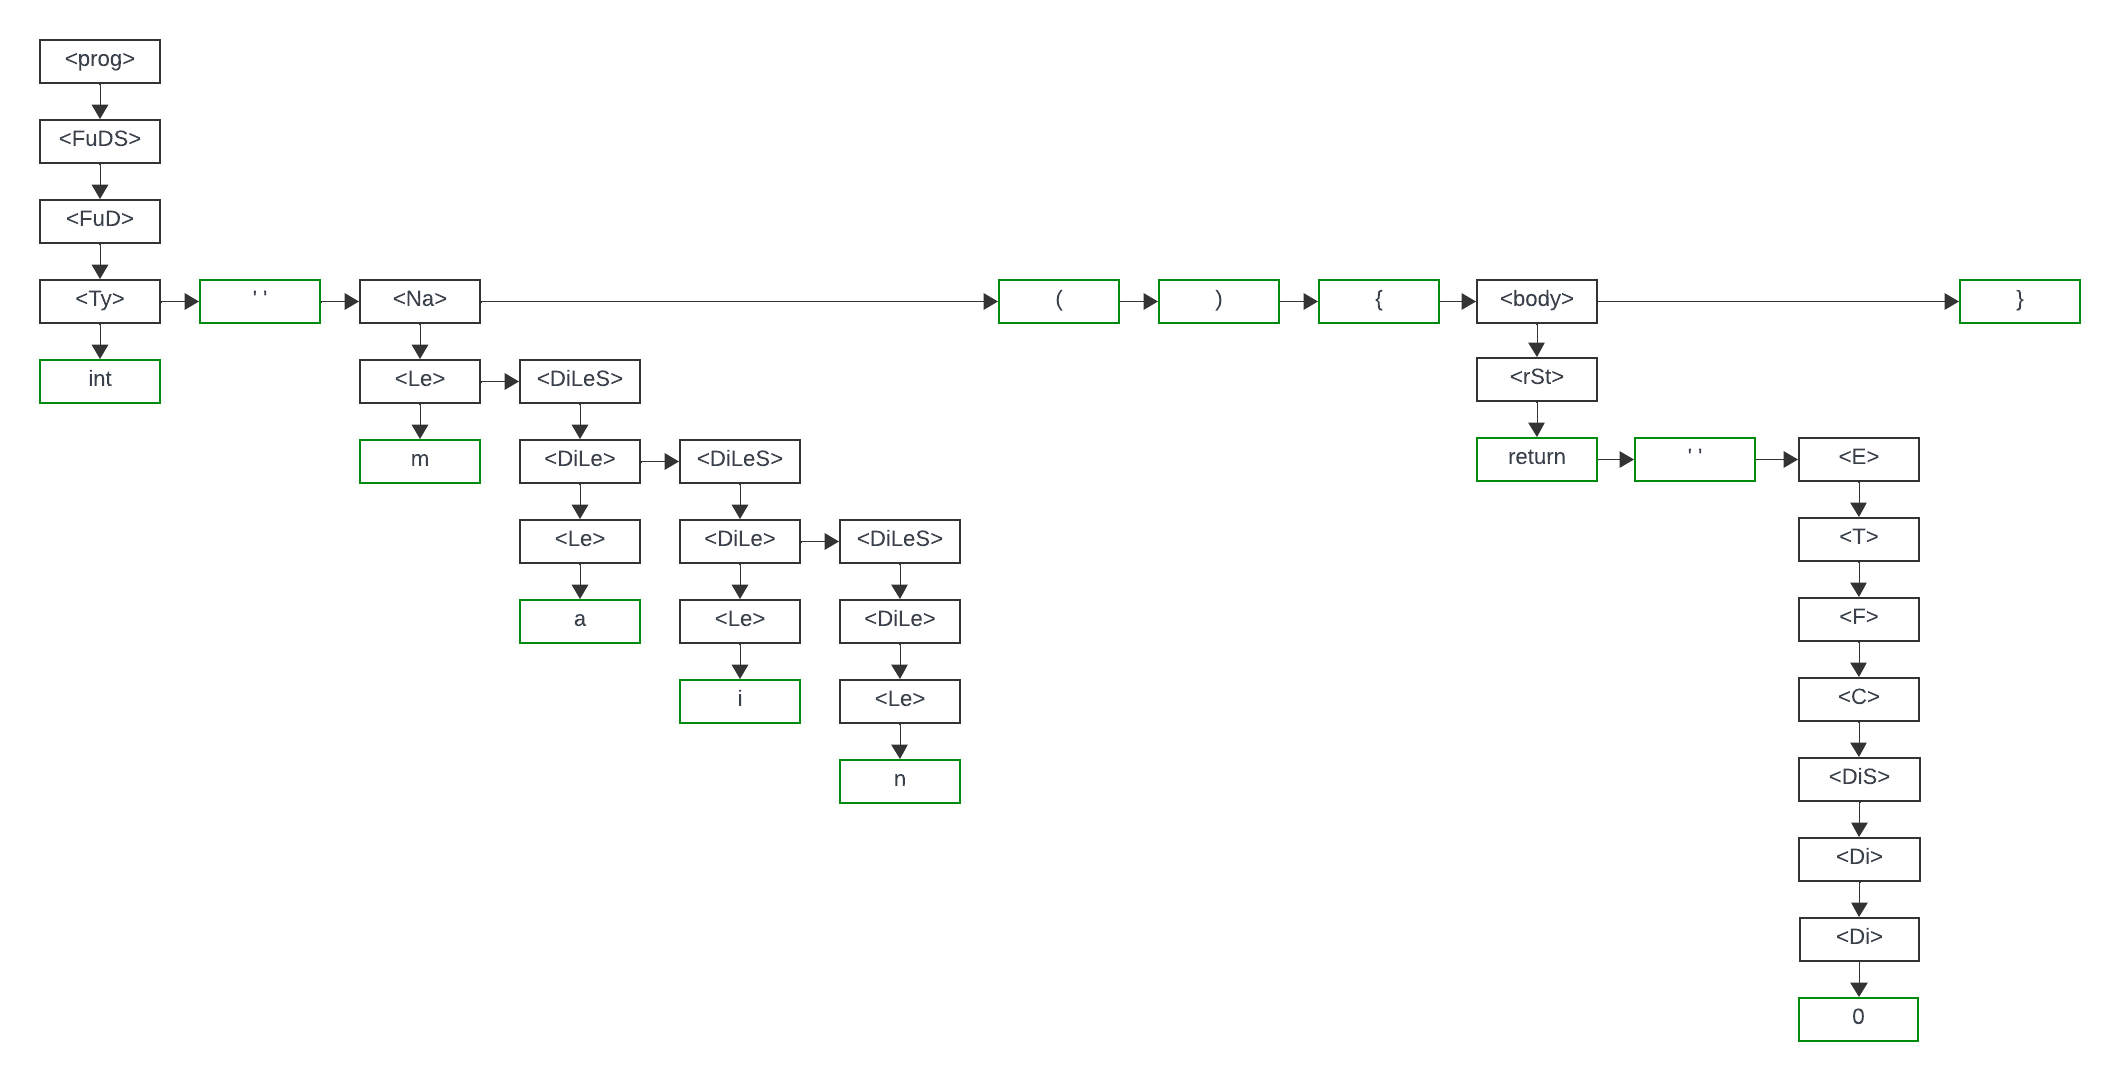
\includegraphics[width=\linewidth]{parseTree.png}
    \caption{the parse tree of the shortest functional C0 code.}
    \label{figure 6}
\end{figure}
